 \documentclass{report}
 
\usepackage[utf8]{inputenc} 
\usepackage[T1]{fontenc}      
\usepackage[top=2.0cm, bottom=3cm, left=3.0cm, right=3.0cm]{geometry}
\usepackage{graphicx}
\usepackage{wrapfig}
\usepackage{amsmath,esint }
\usepackage{amssymb}
\usepackage{esvect}
\graphicspath{{figures/}{../figures}}

\newcommand*\dif{\mathop{}\!\mathrm{d}}
\newcommand*\diver{\mathop{}\!\mathrm{div}}
\newcommand*\grad{\mathop{}\!\mathrm{grad}}

\begin{document}

\section*{Modèle de Drude $\bullet\bullet\bullet$}

En 1900, Paul Drude proposa un modèle permettant d'expliquer les propriétés de conduction électrique et thermique des métaux. Dans ce modèle, on considère que les électrons de conduction forment un gaz de particules classiques de masse $m$ et de charge $-e$, auquel on applique les méthodes issues de la théorie cinétique des gaz. Les électrons effectuent des collisions, considérées comme instantanées. Ils sont supposés indépendants (pas d'interaction électron-électron entre les collisions). Drude attribua les collisions aux chocs entre les électrons et les ions, plutôt qu'aux chocs entre les électrons entre eux comme pour un gaz ordinaire. À l'issue d'une collision, la vitesse de l'électron a une direction aléatoire (pas de direction privilégiée), et une valeur liée à la température à l'endroit où a lieu la collision.

\vspace{0,4cm}

Le paramètre fondamental introduit par Drude est un temps de relaxation, $\tau$ : pour un électron donné, la probabilité de subir une collision pendant un intervalle de temps infinitésimal $dt$ est $dt/\tau$. L'objectif de cet exercice est d'estimer la conductivité d'un métal en fonction de ce temps $\tau$ et de la densité électronique $n$, propres à chaque métal. 

\begin{itemize}
	
	\item[$\spadesuit$]	 On note $N_0$ le nombre total d'électrons dans le métal. Montrer que le nombre d'électrons n'ayant subi aucune collision à un instant $t$ s'écrit $N(t)=N_0\cdot\exp(-t/\tau)$.
	
	\item[$\spadesuit$]	 Montrer que la probabilité pour un électron de subir son premier choc entre $t$ et $t+dt$ est $dp=\frac{dt}{\tau}\cdot\exp(-t/\tau)$. En déduire que $\tau$ correspond au temps moyen entre deux collisions.
	
	\item[$\spadesuit$] On soumet le métal à un champ de force extérieur, et on note $\vec{F}(t)$ la force subie par chaque électron. Comment varie la quantité de mouvement de la totalité des électrons $\vec{P}(t)$ entre $t$ et $t+dt$ ?
	
	\item[$\spadesuit$] En déduire une équation différentielle vérifiée la vitesse moyenne d'un électron $\vec{v}=\vec{P}/(mN_0)$. Quel est l'effet moyen des collisions sur la trajectoire d'un électron ?
	
	\item[$\spadesuit$] On applique au métal un champ électrique uniforme de pulsation $\omega_0$, que l'on note en notation complexe : $\vec{E}(t)=E_0\exp(-i\omega_0t)$. En appliquant le résultat précédent, calculer la densité de courant $\vec{j}$ en fonction de $m$, $e$, $\tau$ et du nombre d'électrons par unité de volume $n$. En déduire l'expression de la conductivité $\gamma(\omega)$ du métal.
	
	\item[$\spadesuit$] En admettant que chaque atome du métal libère un électron de conduction, calculer un ordre de grandeur de $n$.
	
	\item[$\spadesuit$] La résistivité statique du cuivre est mesurée à 273K est $\rho=1,56\cdot10^{-8}\Omega$.m. Calculer le temps de relaxation $\tau$. 
	
	\item[$\spadesuit$] A $t=0$, on applique un champ $\vec{E}$ constant aux électrons du conducteur. Quelle est l'évolution de la vitesse moyenne au cours du temps ? 
\end{itemize}

\newpage

\section*{\textit{Correction Modèle de Drude}}

\begin{itemize}
	
	\item[$\spadesuit$] Entre $t$ et $t+dt$, le nombre d'électrons ayant subi une collision est $N(t)\frac{dt}{\tau}$ : en effet, à $t$ il reste $N(t)$ électrons n'ayant pas collisioné et parmi eux, une proportion $\frac{dt}{\tau}$ va subit une collision durant $dt$. A noter que cela est valable dans le cadre de la loi des grand nombre, qui est largement validée ici au vu des quantité d'électrons dans un métal.
	
	On en déduit alors que le nombre d'électrons n'ayant pas collisioné à $t+dt$ est :
	\begin{align*}
		N(t+dt) = N(t) - N(t)\frac{dt}{\tau}
	\end{align*}
	On tombe sur l'équation différentielle classique de la désintgration radioactive, donnée par $\dot{N}(t)=-\frac{1}{\tau}N(t)$.En intégrant, on trouve la relation voulue.
	
	\item[$\spadesuit$] La probabilité pour un électron de ne pas subir de collision jusqu'à l'instant $t$ correspond au nombre total d'électrons n'yant pas subi de collision sur le nombre total d'électrons, soit $N(t)/N_0=\exp(-t/\tau)$. 
	
	La probabilité $dp$ pour un électron de subir une collision entre $t$ et $t+dt$ correspond à la \textit{probabilité de ne pas avoir subi de collision jusqu'à} $t$ ET à la \textit{probabilité de subir une collision entre $t$ et $t+dt$}, soit le produit de probabilité :
	\begin{align*}
		dp = \exp(-t/\tau)\cdot\frac{dt}{\tau}
	\end{align*}
La valeur moyenne du temps de collision correspond à la somme des temps $t$ durant laquelle il y a eu collision multiplié par la probabilité de collision entre $t$ et $t+dt$ :
	\begin{align*}
		\bar{t}=\int_0^{\infty}tdp=\int_0^{\infty} t\exp(-t/\tau)\cdot\frac{dt}{\tau}=\tau
	\end{align*}
	
	\item[$\spadesuit$] Soit $N_0$ le nombre total d'électrons. Entre $t$ et $t+dt$, il y a eu $dtN_0/\tau$ qui ont subi une collision. La quantité de mouvement de tous ces électrons est donc perdue. D'autre part, entre $t$ et $t+dt$ chaque électron est soumis à la force $\vec{F}(t)$, faisant changer la quantité de mouvement totale de $N_0F(t)dt$. Finalement, il vient :
	\begin{equation}
		\vec{P}(t+dt)=\vec{P}(t)-\frac{dt}{\tau}\vec{P}(t)+N_0\vec{F}dt
	\end{equation}
	
	\item[$\spadesuit$] On en déduit la vitesse moyenne d'un électron, définie par $\vec{v}(t)=\vec{P}/(mN_0)$ :
	\begin{align*}
		\frac{d\vec{v}}{dt}=\frac{\vec{v}}{\gamma}+\vec{F}(t)
	\end{align*}
	où $\gamma=m/\tau$.
	
	\item[$\spadesuit$] La force subie par les électrons est la force de Lorentz : $\vec{F}=-eE_0\exp(-i\omega t)$. L'équation précédente devient :
	\begin{align*}
		-i\omega\vec{v}=-\frac{e}{m}\vec{E_0}-\frac{\vec{v}}{\tau}
	\end{align*}
	On en déduit :
	\begin{align*}
		\vec{v}=\frac{e\tau}{m}\frac{E_0}{i\omega\tau-1}
	\end{align*}
	En introduisant la conductivité $\gamma$, $\vec{j}=\gamma \vec{E}$, où $\vec{j}=-ne\vec{v}$, on trouve :
	\begin{align*}
		\gamma(\omega)=\frac{ne^2\tau}{m}\frac{1}{1-i\omega\tau}
	\end{align*}
	
	\item[$\spadesuit$] Dans un métal, qui est un réseau cristallin, il y a typiquement un électron tous les Angstrom, soit tous les $10^{-10}$m. On obtient des densités typiques de $10^{30}$ atomes par m$^3$.
	
	\item[$\spadesuit$] La résistivité statique correspond à une fréquence qui tend vers 0, cad :
	\begin{align*}
		\rho = \frac{1}{\gamma}=\frac{m}{ne^2\tau}
	\end{align*}
	On trouve donc $\tau\simeq10^{-14}$s.
	
\end{itemize}

\newpage

\newpage

\section*{Conduction dans un semiconducteur bidimensionnel $\bullet\bullet\circ$}
 
Les techniques récentes de microfabrication permettent de créer à partir de semiconducteurs dopés (cristaux d'arsenure de gallium) des conducteurs où les électrons sont quantiquement confinés dans un plan : leur déplacement, et donc la condution électrique, sont parfaitement bidimensionnels. On s'intéresse au conducteur 2D rectangulaire de largeur $W$ et de longueur $L$ ci-dessous, contenant un total de $N_0=n_s\times W\times L$ électrons, où $n_s$ est la densité surfacique d'électron.

\begin{figure}[h!]
\centering
		\includegraphics[scale=0.5]{2DEG_square.pdf}
\end{figure}

On admet que les électrons dans ce plan se comportent comme un gaz parfait : ils n'interagissent pas entre eux et ne sont soumis qu'à champ électrique $\vec{E}$ uniforme lorsque un opérateur impose une différence de potentiel $V_1-V_2$. Ils subissent néanmoins des collisions avec les impuretés du réseau cristallin, à l'issue desquelles ils ont une direction et une vitesse aléatoire. On admet que durant un temps $dt$, la probabilité pour un électron de subir une collision est $dp = dt/\tau$, où $\tau$ est un paramètre imposé par la qualité du réseau cristallin.

L'objectif de l'exercice est de déterminer les propriétés de conduction d'un tel matériau, en fonction de ses caractéristiques $n_s$ et $\tau$.

\begin{itemize}

	\item[$\bowtie$] Relier le courant surfacique $\vec{j_s}$ à la densité surfacique $n_s$ d'électron et leur vitesse moyenne $\vec{v}$. Relier ensuite $\vec{j_s}$ avec $I$ et $W$.

	\item[$\bowtie$] A l'instant $t$, $P(t)=mN_0v(t)$ la quantité de mouvement totale des électrons. En effectuant un bilan de quantité de mouvement, montrer qu'en régime permanent on a :
	\begin{align*}
		\vec{v}=-\frac{e\tau}{m}\vec{E}
	\end{align*}
	
	\item[$\bowtie$] L'opérateur impose une différence de potentiel $U=V_1-V_2$, générant un courant total $I$ réparti uniformément dans le conducteur. En déduire la résistance $R$ du conducteur en fonction de $n_s$, $\tau$, $L$ et $W$.
	
	\item[$\bowtie$] Pourquoi appelle t-on $R_\boxdot=\frac{m}{e^2\tau n_s}$ résistance par carré ?
	
\end{itemize}

On s'interesse à un conducteur bidimensionnel avec une géométrie en "sablier", proposée sur le schéma ci-dessous. Il s'agit d'un "quantum point contact", un dispositif permettant d'étudier les propriétés quantiques des électrons dans les conducteurs.

\begin{figure}[h!]
\centering
		\includegraphics[scale=0.5]{2DEG_QPC.pdf}
\end{figure}

\begin{itemize}

	\item[$\bowtie$] En supposant que la densité de courant est uniforme dans la largeur du conducteur 2D, calculer la résistance totale $R$ de ce conducteur.
	
	\item[$\bowtie$] Calculer la puissance surfacique locale dissipée par effet Joule, $p_s=\vec{j_s}\cdot\vec{E}$, puis la puissance totale $P_J$ dissipée dans le conducteur. A t-on $P_J=RI^2$ ?

\end{itemize}

\newpage

\section*{\textit{Correction Conduction dans un semiconducteur bidimensionnel}}

\begin{itemize}

	\item[$\bowtie$] $\vec{j_s}=-en_s\vec{v}$ et $\vec{j_s}=I/W$.

	\item[$\bowtie$] Entre $t$ et $t+dt$, les électrons ont acquis une quantité de mouvement $-eN_0\vec{E}dt$, mais en ont perdu par collision $-P(t)dp=-P(t)\times dt/\tau$ (comme une fraction $dt/\tau$ d'électrons ont perdu \textbf{en moyenne} leur quantité de mouvement). On a donc :
	\begin{align*}
		P(t+dt) = P(t)-eN_0\vec{E}dt-P(t)\frac{dt}{\tau}
	\end{align*}
	En régime permanent, $P(t+dt) = P(t)$, donc :
	\begin{align*}
		\vec{P}=-eN_0\tau\vec{E}
	\end{align*}
	Et alors :
	\begin{align*}
		\vec{v}=-\frac{e\tau}{m}\vec{E}
	\end{align*}
	
	\item[$\bowtie$] Le courant surfacique est donc :
	\begin{align*}
		\vec{j_s}=\frac{e^2\tau n_s}{m}\vec{E}
	\end{align*}
	
	Et comme $V_1-V_2 = int_1^2\vec{dl}\cdot \vec{E}=E\times L$ et que $I=j_S\times W$, on obtient :
	\begin{align*}
		V_1-V_2 = I\times\frac{m}{e^2\tau n_s}\frac{L}{W}
	\end{align*}
	Donc $R_\boxdot = \frac{m}{e^2\tau n_s}\frac{L}{W}$
	
	\item[$\bowtie$] $R_\boxdot$ ne dépend que du rapport d'aspect du conducteur (qui est rectangulaire) : dans le cas $W=L$, la résistance ne dépend plus des dimensions du conducteur. Pour connaitre la resistance d'un tel conducteur, il suffit de "compter" les carrés composant le conducteur (et faire les lois d'addition de résistance en série et en parallèle) pour en déduire la résistance totale du conducteur.
	
	\item[$\bowtie$] On note $x$ la dimsension le long du conducteur (selon $l$) et on décompose le conducteur en 3 parties : la première partie du sablier, le carré central et la seconde partie en sablier, notées 1, 2 et 3.
	
	Dans la partie $1$, on a $j_s=I/(w-ax)$, avec $a=\frac{l}{W-d}$. Comme on a toujours $\vec{j_s}=\frac{e^2\tau n_s}{m}\vec{E}$, on obtient :
	\begin{align*}
		\Delta V_1=\frac{m}{e^2\tau n_s}\int_{x=0}^{x=l}dxj_s(x)=\frac{m}{e^2\tau n_s}\times\frac{I}{a}\ln\left(\frac{w}{d} \right) 
	\end{align*}
	où $\Delta V_1 = V_1-V(x=l)$ est la chute de tension dans la partie 1. On a $\Delta V_1+\Delta V_2+\Delta V_3=V_1-V_2 = E\times (2l+d) $.
	
	Finalement, on obtient :
	\begin{align*}
		R_1=\frac{m}{e^2\tau n_sa}\ln\left(\frac{w}{d} \right) =\frac{R_\boxdot}{a}\ln\left(\frac{w}{d} \right)
	\end{align*}
	
	Comme la résistance centrale est une résistance "carrée", on a $R_2=R_\boxdot$. Enfin, par symétrie, on a $R_1=R_3$. Donc :
	\begin{align*}
		R = R_1+R_2+R_3 = R_\boxdot\left(\frac{2}{a}\ln\left(\frac{w}{d} \right)+1 \right) 
	\end{align*}
	
	
	\item[$\bowtie$] $p_s=\vec{j_s}\cdot\vec{E}=\frac{I}{l(x)}\times\frac{V_1-V_2}{2l+d}$, où $l(x)$ est la largeur du conducteur en $x$. 
	
	La puissance totale est donc :
	\begin{align*}
	P_J = \iint dx dy\times p_s = \int_{0}^{2l+d} dx l(x)\times\frac{I}{l(x)}\times\frac{V_1-V_2}{2l+d} = (V_1-V_2)\times I= RI^2
	\end{align*}

\end{itemize}

\newpage

\section*{Résistance d'une plaque infinie $\bullet\bullet\bullet$}

On considère une plaque métallique de conductivité $\gamma$, infinie dans le plan $xy$ et d'épaisseur $e$ selon $z$. Cette plaque est connectée à deux fils de même métal (et donc de même conductivité $\gamma$) en $A$ et $B$, séparés l'un de l'autre de la distance $d$. Ces deux fils peuvent être assimilés à des cylindres de rayon $a$ et de longueur $l$. 

\begin{figure}[h!]
\centering
		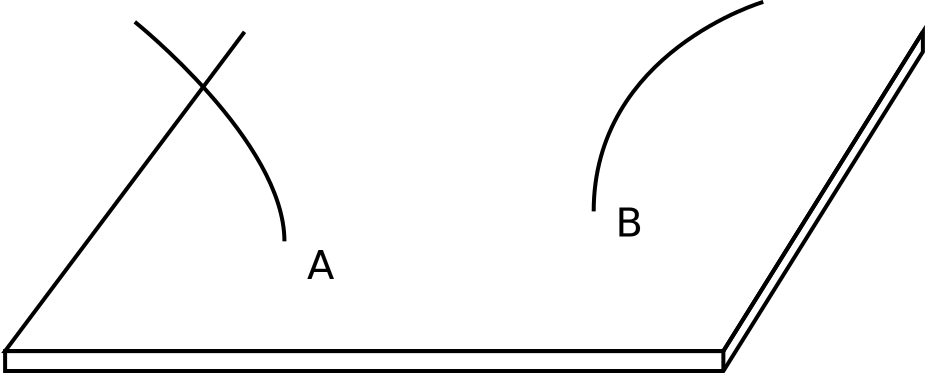
\includegraphics[scale=0.3]{plaque.pdf}
\end{figure}

\begin{itemize}

	\item[$\heartsuit$] Quelle est la résistance de chaque fil ? 
	
	\item[$\heartsuit$] A l'aide des symétries du problème, proposez une expression pour la densité de courant à l'intérieur de la plaque. 
	
	\item[$\heartsuit$] En déduire la résistance équivalente entre les points $A$ et $B$. Quelle est la résistance totale du dispositif ?
	
	\item[$\heartsuit$] On considère désormais que les fils sont reliés ne sont plus reliés à une plaque mais à un volume du même métal, c'est-à-dire, $e\longrightarrow\infty$. Par le même raisonnement, en déduire la résistance équivalente. 

\end{itemize}

\newpage

\section*{\textit{Correction Résistance d'une plaque infinie}}

\begin{itemize}

	\item[$\heartsuit$] Résistance classique d'un cylindre : $R=L/(\gamma\pi a^2)$.
	
	\item[$\heartsuit$] Isolons le câble arrivant en $A$. Par symétrie, le courant $I$ partira dans tous les directions. La densité de courant va s'écrire en un point $M$ :
	\begin{align*}
		\vec{j_A}=\frac{I}{2\pi e }\frac{\vec{AM}}{\|\vec{AM} \|^2}
	\end{align*}
	C'est une décroissance typique en $1/r$, où $r=AM$.
	On effectue le même raisonnement pour la source de courant en $B$, mais où la source de courant est $-I$. Par superposition, la densité de courant totale est alors :
	\begin{align*}
		\vec{j}=\frac{I}{2\pi e }\left[ \frac{\vec{AM}}{\|\vec{AM} \|^2} - \frac{\vec{BM}}{\|\vec{BM} \|^2}\right] 
	\end{align*}
	
	\item[$\heartsuit$] En intégrant la relation $\vec{j}=\gamma\vec{E}$ le long du chemin $AB$, dont la coordonnée sera donnée par $x$, en faisant varier $x$ de $a$ à $d-a$ (pour éviter une divergence de la densité de courant) :
	\begin{align*}
		\int_a^{d-a}dx j(x)=\frac{I}{2\pi e}\int_a^{d-a}dx\left(\frac{1}{x}+\frac{1}{d-x} \right) =\gamma\int_a^{d-a}dxE=-\gamma\int_a^{d-a}dx\frac{dV}{dx}
	\end{align*}
	
	\textit{Remarque} : Lorsque $M$ est strictement contenu sur le segment $AB$, on a : $\vec{BM} = -\|BM\|\vec{e}_x=-(d-a)\vec{e}_x$ où $\vec{e}_x$ est le vecteur normé orientant ce segment. 
	
	On trouve alors :
	\begin{align*}
		\Delta V = \frac{I}{\pi e\gamma}\log\left(\frac{d-a}{a} \right) 
	\end{align*}

	\item[$\heartsuit$] En se plaçant en coordonnées sphériques, on a :
	\begin{align*}
		\vec{j}=\frac{I}{2\pi}\left[ \frac{\vec{e_r}}{\|\vec{AM} \|^2} - \frac{\vec{e_r}}{\|\vec{BM} \|^2}\right] 
	\end{align*}
	Attention, il y a un facteur 2 par rapport à la surface d'une sphère car il s'agit de demi-sphères.
		On trouve alors :
	\begin{align*}
		\Delta V = \frac{I}{\pi \gamma}\frac{d}{a(d-a)}
	\end{align*}
	
\end{itemize}

\newpage

\section*{Paratonnerre $\bullet\circ\circ$}

Lorsque le courant de foutre d'un impact direct sur un paratonnerre s'écoule par la prise de terre d'une installation, de fortes surtensions peuvent apparaître. La résistance de prise de terre ne doit pas dépasser 30$\Omega$. Considérons une prise de terre constituée d'une demi-sphère métallique pleine, de rayon $a$ et placée dans un sol de conductivité $\gamma\approx10^{-2}$S.m$^{-1}$. Le courant de foudre d'intensité $I$ arrive sur la tige paratonnerre fixée au centre $C$ de l'hémisphère.

\begin{figure}[h!]
\centering
		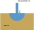
\includegraphics[scale=1.5]{EM1.pdf}
\end{figure}

\begin{itemize}
	
	\item[$\diamondsuit$] Quelle est la densité de courant $\vec{j}$ dans le sol pour $r>a$ ? Déterminer alors le potentiel $V(r)$, en supposnat que celui-ci est nul à l'infini. 
	
	\item[$\diamondsuit$] Déterminer la valeur du rayon $a$ pour laquelle la valeur de la résistance de la prise de terre ne dépasse pas 30$\Omega$.
	
	\item[$\diamondsuit$] La tension de pas est définie comme la différence de potentiel entre 2 points de la surface du sol distants de 1 mètre et situés sur la même droite issue du centre $C$ de l'hémisphère. Calculer cette tension de pas $V_p$ pour un courant de 50kA, à une distance de 10m puis de 100m.
	
	\item[$\diamondsuit$] Sachant que la résistance entre les deux pieds d'une personne est de l'ordre de 2500$\Omega$, et que l'intensité létale pour un corps humais est de 25mA, une personne est-elle en sécurité à 10m ? A 100m ? 
	
\end{itemize} 

\newpage


\section*{\textit{Correction Paratonnerre}}


\begin{itemize}

	\item[$\diamondsuit$] Les lignes de champs sont radiales cad $\vec{j}=j(r)\vec{e_r}$. On a donc :
\begin{align*}
	\vec{j}(r)=\frac{I}{2\pi r^2}\vec{e_r}
\end{align*}
On en déduit :
\begin{align*}
	\dif V=-E(r)dr=\frac{-I}{2\pi r^2\gamma}dr
\end{align*}
Par intégration, on trouve :
\begin{align*}
	V(r)=\frac{I}{2\pi r\gamma}
\end{align*}

	\item[$\diamondsuit$] Le potentiel de l'hémisphère est donc simplement :
\begin{align*}
	U=\frac{I}{2\pi a\gamma}
\end{align*}
La résistance est donc tout simplement $R=\frac{1}{2\pi a \gamma}$. On trouve qu'elle ne dépasse pas 30$\Omega$ si $a>53$cm.

	\item[$\diamondsuit$] La tension de pas vaut, si $d=1$m :
	\begin{align*}
		V_p(r)=V(r)-V(r+d)=\frac{I}{2\pi \gamma r(r+d)}
	\end{align*}
On trouve que $V_p(10m)=7,2kV$ et  $V_p(100m)=79V$

	\item[$\diamondsuit$] Le courant qui traverse la personne est $i=V_p/R$. On trouve i(10)=2,9A et i(100)=32mA.
\end{itemize}

\end{document}